\documentclass{article}

\usepackage{graphicx}
\usepackage{setspace}
\usepackage{listings}
\usepackage{color}
\usepackage{circuitikz}
\usepackage{float}
\usepackage[title]{appendix}
\usepackage{etoolbox}        %Used to add colons after Appendix labels

%From etoolbox. However, subsections will print with a colon ater as well
%(apparently - I haven't tested this)
\patchcmd{\appendices}{\quad}{: }{}{}

% Set margins to 0.5inch
\usepackage[margin=1in]{geometry}


\title{ECE 210 - Combinational Logic Design \\ Lab 3}
\date{2018-11-07}
\author{Radomir Wasowski \\ wasowski@ualberta.ca
        \and David Lenfesty \\ lenfesty@ualberta.ca}

\setcounter{tocdepth}{2} % Show subsections

\definecolor{dkgreen}{rgb}{0,0.6,0}
\definecolor{gray}{rgb}{0.5,0.5,0.5}
\definecolor{mauve}{rgb}{0.58,0,0.82}

\lstset{basicstyle=\small,
        keywordstyle=\color{mauve},
        identifierstyle=\color{dkgreen},
        stringstyle=\color{gray},
        numbers=left
        }

\begin{document}

\pagenumbering{gobble}
\doublespacing
\maketitle
\newpage

\singlespacing

\section{Abstract}

When a person interacts with a digital system, it is sometimes necessary to convey certain information about the system to that person. Using a display is an effective way to make that information accessible in an easy to parse format.
By using logic gates to implement a 7-segment display that can directly output the single-digit hexadecimal value of a sensor,
a simple user interface can be built.

\section{Introduction}

In this lab, we were tasked with designing VHDL circuits that were able to update a 7-segment display
in order to display a hexadecimal digit.
In parts 1 \& 2, we were asked to do this using structural and behavioural logic, respectively.
Parts 3 \& 4 tasked us with using the display that was just designed in order to count from 0x0 to 0xF, on one or two separate displays.

\section{Design}

\paragraph{Part 1:}

Because many characters, when displayed on a 7-segment display, share common elements,
it is relatively trivial to combine logic signals using minterms or maxterms.
Based on the 4-bit input, a separate Karnaugh map for each segment of the display was constructed. After simultaneously analyzing all of the K-Maps for similar groups of inputs, a series of logical outputs
were found which would show all of the  desired output numbers/letters with the smallest number of network inputs and logic gates. These values were then connected to the appropriate display segments.
Performing such an analysis reduced the number of discrete logic elements vastly.
Once these signals were found, they were transcribed into a VHDL file,
to be uploaded to an FPGA for testing. The code used can be found in Appendix A.

\paragraph{Part 2:}

Instead of defining all of the logic gates in a network manually, VHDL also supports
behavioural programming.
This style is different in that the synthesizer will decide how to implement
the code in logic, rather that making the programmer do the heavy lifting.
Utilizing a case statement in code, the programmer defines the values in the output vector for each possible input combination
without having to worry exactly how the logic should work in hardware.
While this method is easier for the designer, it does take away some of the control over how the circuit operates.

\paragraph{Part 3:}

Using one of the built-in clocks on the FPGA board, it is fairly simple to implement an upcounter with a specific delay.
The signal from the clock can be sent to an internal counter which can
be divided to fit a 1 second signal, which can then be stored in another counter. This can finally be output directly to the 7-segment display.

\paragraph{Part 4:}

Beyond the 7 inputs for the segments, the display used also has a line for enabling/disabling. The FPGA board in the lab has two displays mounted to it, with both displays connected to the same enable line in complement to eachother (ie. only one display can be on at a time). If the signal controlling which of the two displays are on is inverted 
extremely quickly (\textgreater\ $\sim$200Hz), we can take advantage of the limitations
of the human eye to make it appear as if both displays are on at the same time.
This functionality can easily be implemented by using behavioural logic to
toggle the control signal on the positive edge of every clock cycle.

\section{Results}

For all parts of this lab, the display behaved as expected,
showing the correct hexadecimal digit for the 4-bit input.
Using the example code made available on eclass, the counter updated once a second, and we were able
to show this information on both screens at once.
Pictures of the display in action can be found in Appendix B in Figures 1 and 2.

\section{Discussion \& Conclusion}

While structural code in VHDL allows a designer to design extremely efficient and useful
logic circuits, behavioural code allows the designer to offload much of the tedious or complex
portions of the design onto the synthesizer.
This means that new features and functionality can be quickly and simply designed, while more time/space sensitive applications which require more significant analysis and optimization can still be implemented in the language.

%\newpage
\vskip 2cm

\begin{appendices}

\section{Code}

\begin{lstlisting}[language=VHDL]
entity part1 is
    Port ( sw : in STD_LOGIC_VECTOR (3 downto 0);
           out_7seg : out STD_LOGIC_VECTOR (6 downto 0);
           CC : out STD_LOGIC);
end part1;

architecture Behavioral of part1 is
    signal I : STD_LOGIC_VECTOR (18 downto 1);
begin
     CC <= '0';

     I(1)  <= not sw(2) and not sw(0);
     I(2)  <=  not sw(3) and sw(1) and sw(0);
     I(3)  <= sw(3) and not sw(1) and not sw(0);
     I(4)  <= sw(3) and not sw(2) and not sw(1);
     I(5)  <= sw(2) and sw(1) and not sw(0);
     I(6)  <= sw(3) and sw(2) and sw(1);
     I(7)  <= not sw(3) and sw(2) and sw(0);
     I(8)  <= not sw(3) and not sw(1) and not sw(0);
     I(9)  <= sw(3) and not sw(1) and sw(0);
     I(10) <= not sw(2) and not sw(1);
     I(11) <= not sw(2) and sw(1) and sw(0);
     I(12) <= sw(3) and not sw(2) and sw(1);
     I(13) <= not sw(3) and sw(2);
     I(14) <= sw(2) and not sw(1) and sw(0);
     I(15) <= not sw(3) and not sw(2) and not sw(0);
     I(16) <= sw(3) and sw(2);
     I(17) <= not sw(3) and sw(2) and not sw(1);
     I(18) <= not sw(2) and sw(1);
     
     out_7seg(0) <= I(1) or I(2) or I(3) or I(4) or I(5) or I(6) or I(7);
     out_7seg(1) <= I(1) or I(2) or I(8) or I(9) or I(10);
     out_7seg(2) <= I(9) or I(10) or I(11) or I(12) or I(13);
     out_7seg(3) <= I(3) or I(4) or I(5) or I(11) or I(14) or I(15);
     out_7seg(4) <= I(1) or I(3) or I(5) or I(12) or I(16);
     out_7seg(5) <= I(3) or I(4) or I(5) or I(6) or I(8) or I(12) or I(17);
     out_7seg(6) <= I(4) or I(5) or I(6) or I(9) or I(17) or I(18);

end Behavioral;
\end{lstlisting}

\section{Images}

    \begin{figure}[H]
	\centering
        % Mess around with widths later
        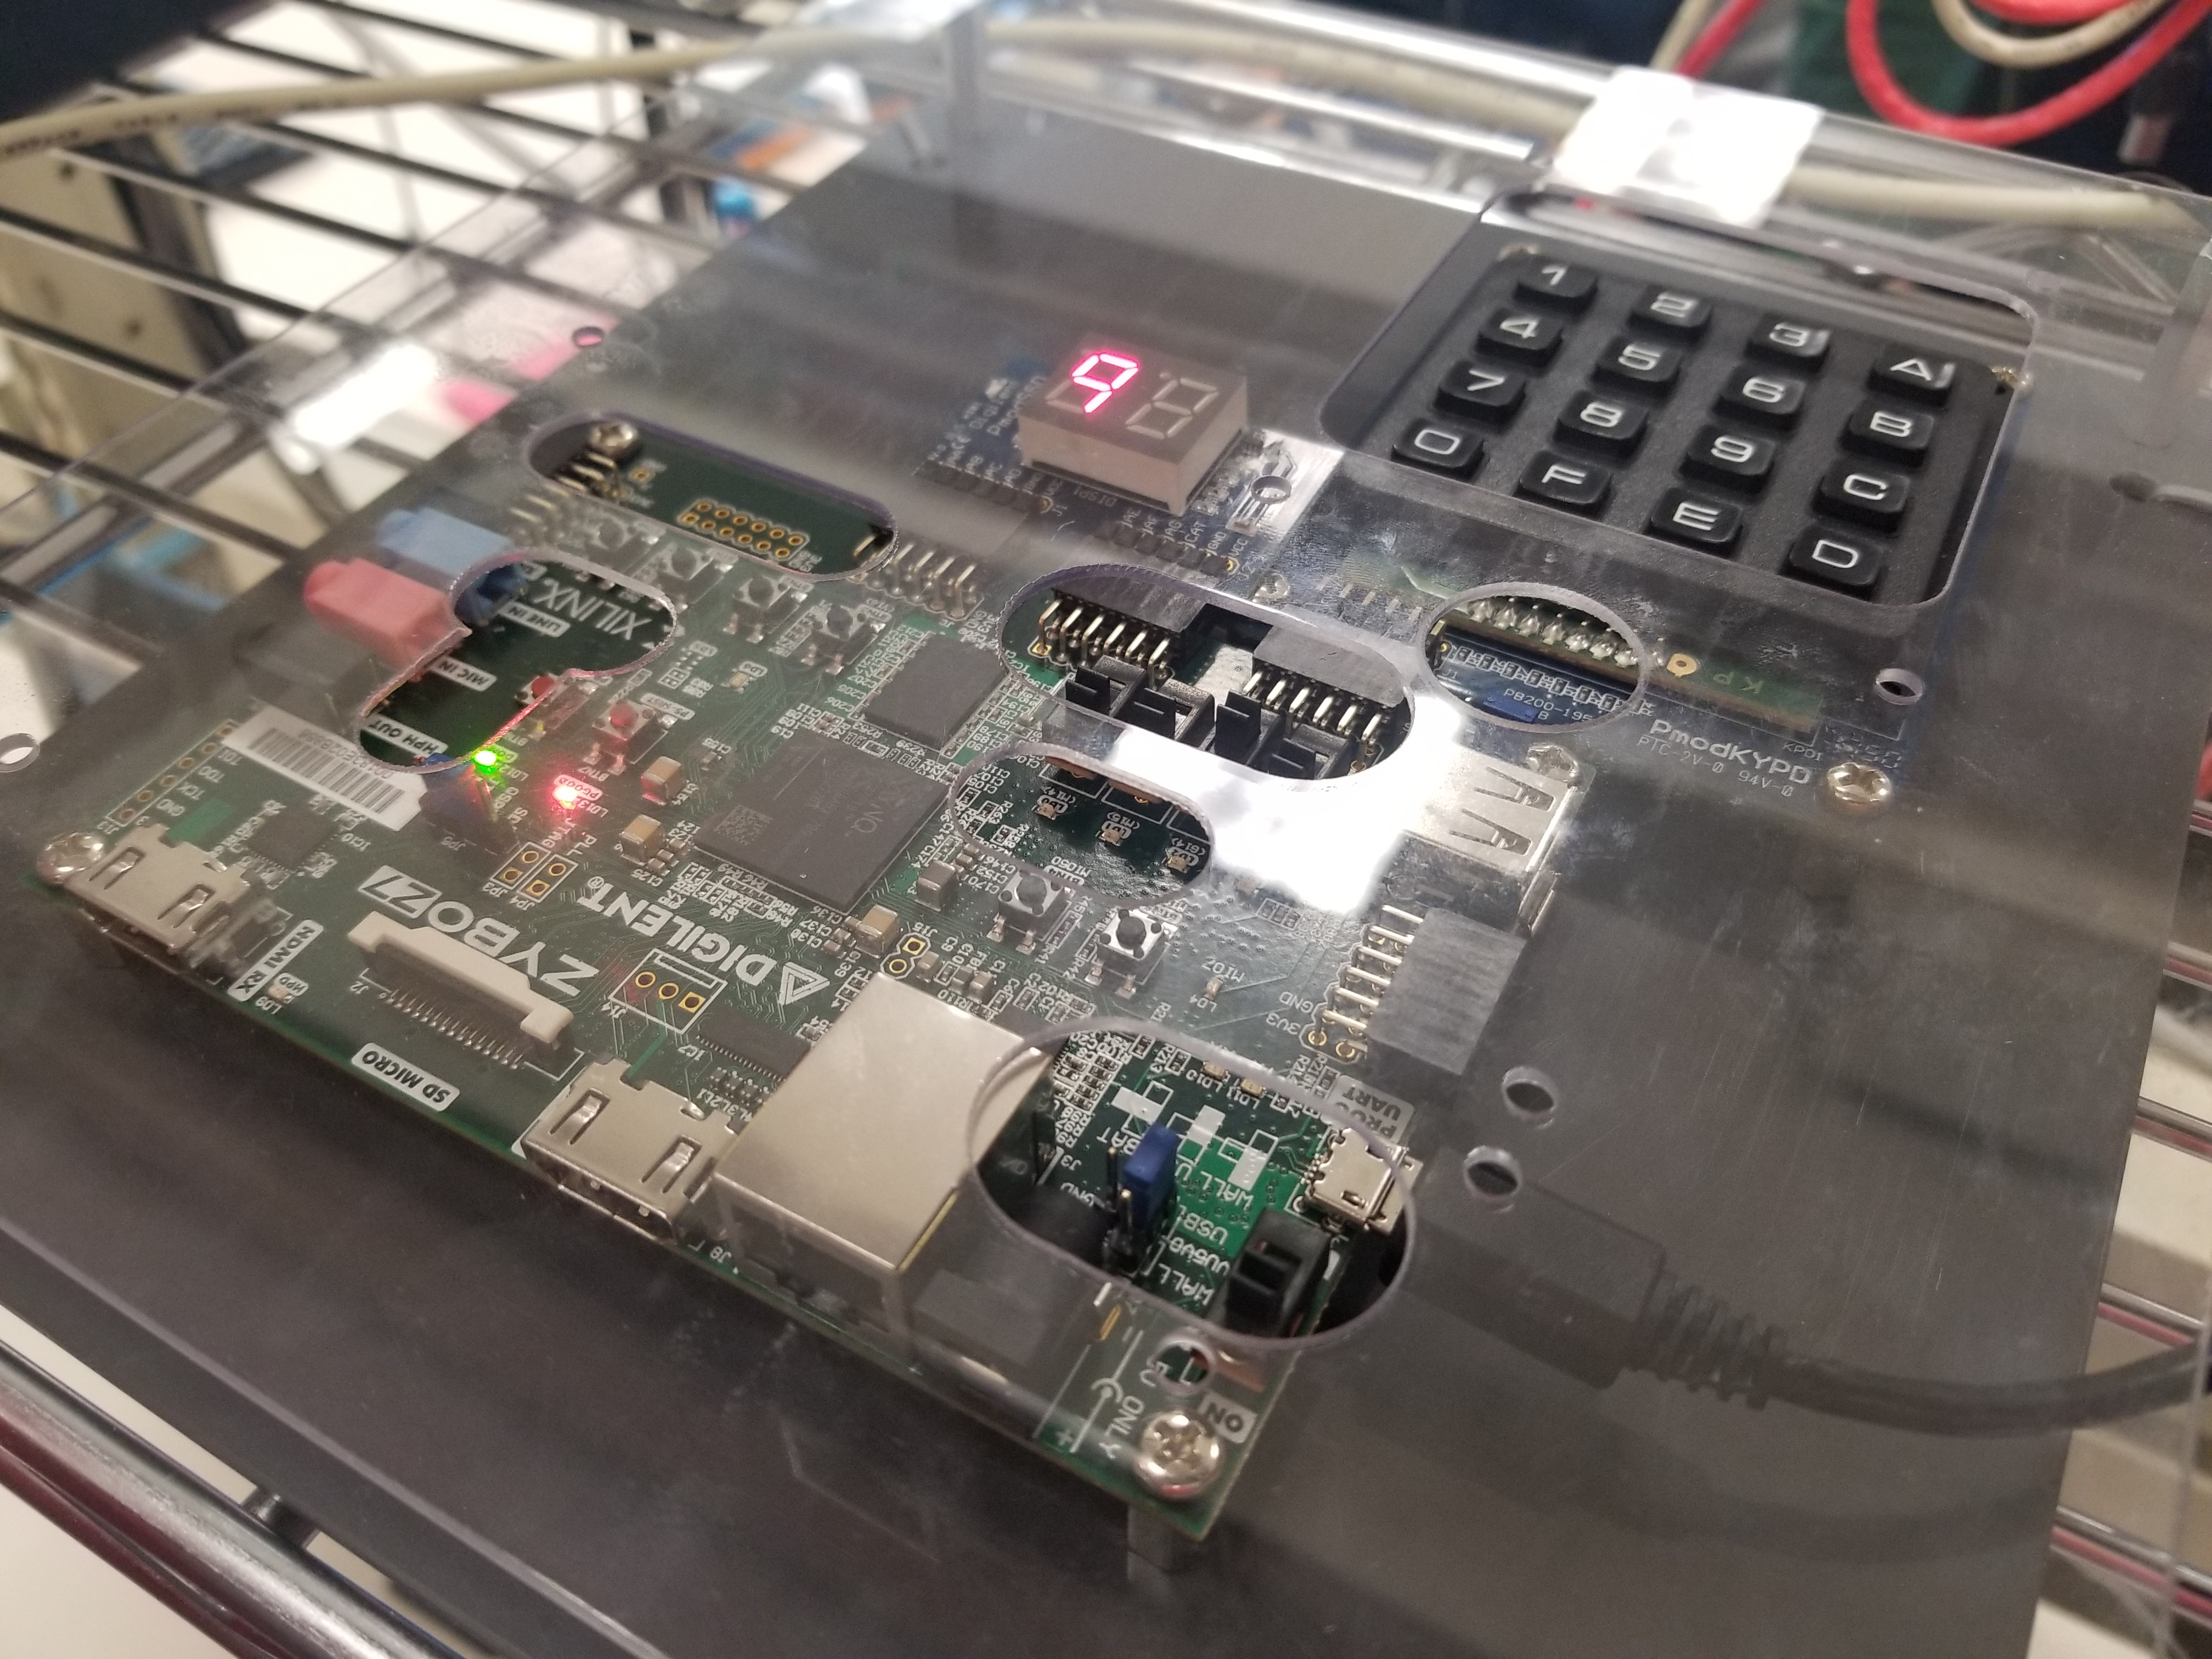
\includegraphics[width=125mm]{display_single.jpg}
        \caption{Single-character hexadecimal display.}
        \label{fig:display_single}
    \end{figure}

    
    \begin{figure}[H]
	\centering
        % Mess around with widths later
        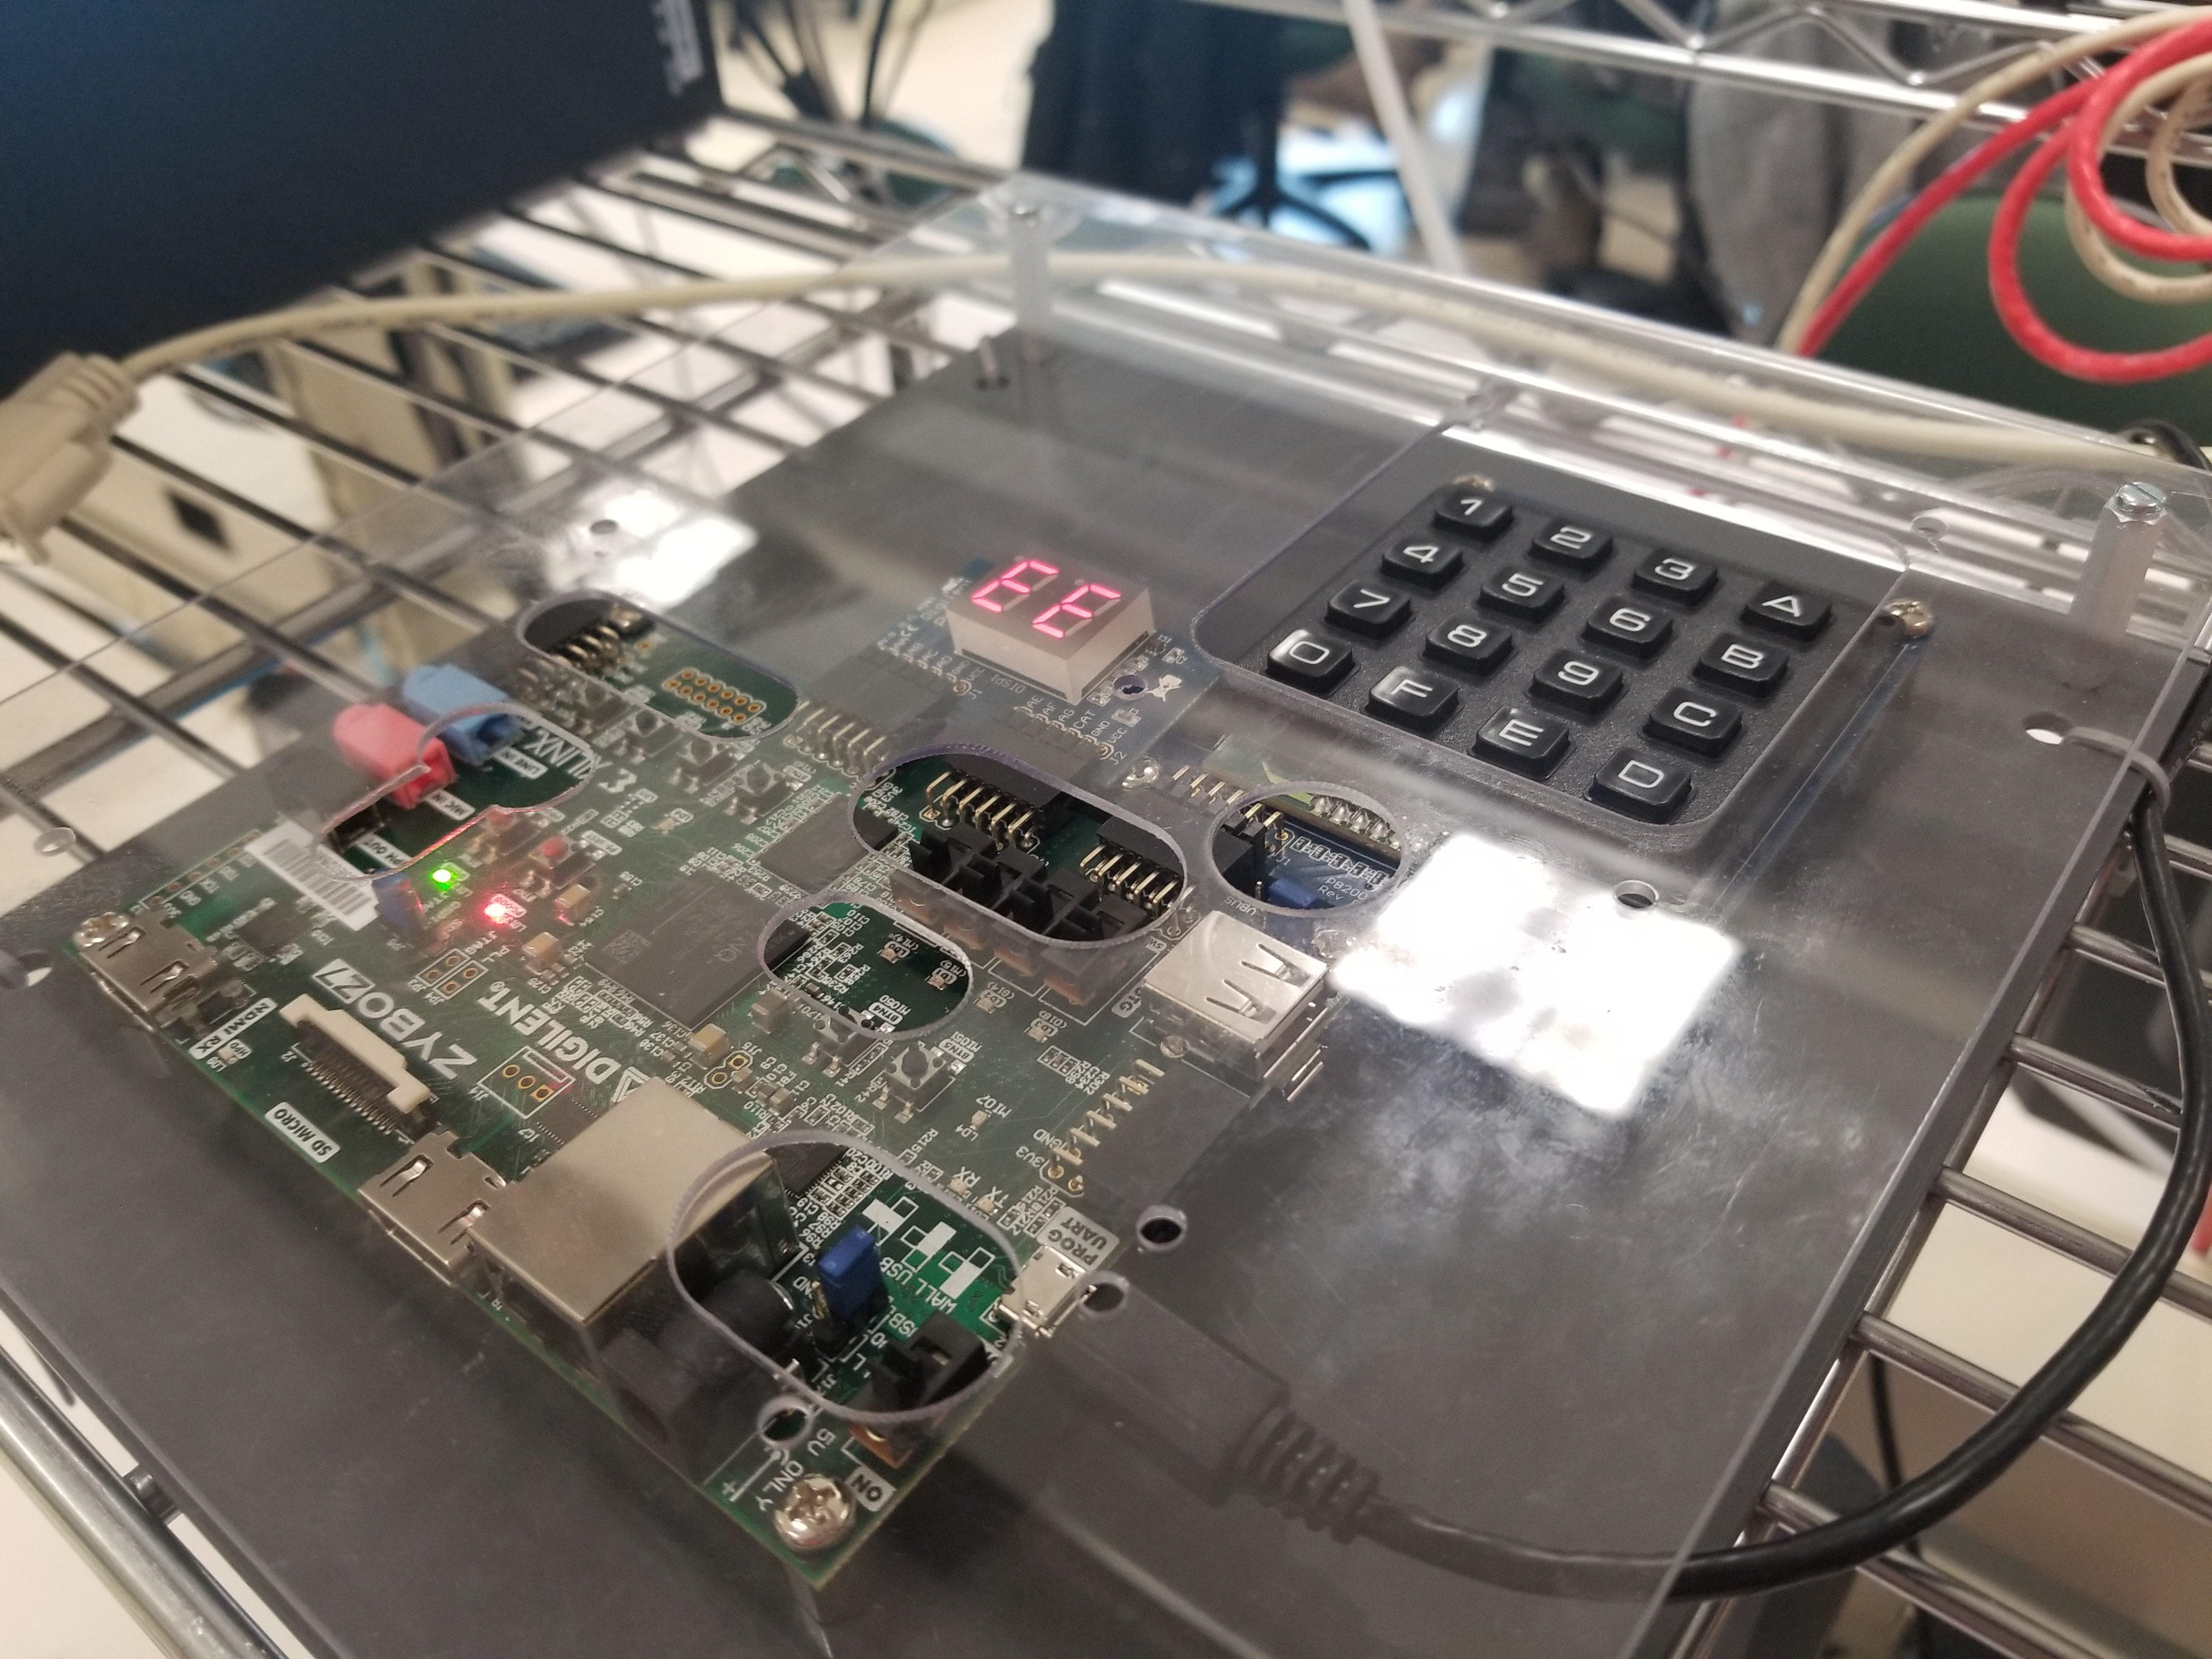
\includegraphics[width=125mm]{counter_dual.jpg}
        \caption{Both displays operating seemingly at the same time.}
        \label{fig:counter_dual}
    \end{figure}
\end{appendices}

\end{document}
